\documentclass[a4paper, 12pt]{scrartcl}
\usepackage[utf8]{inputenc}
\usepackage[english]{babel}

\usepackage{hyperref}
\usepackage{graphicx}

% \usepackage{fancyhdr}
% \pagestyle{fancy}
% \fancyhf{}
% \lhead{WIP 1.3}
% \cfoot{\thepage}

\usepackage[left=2.5cm, right=2.5cm, top=2.0cm]{geometry}

% \usepackage{setspace}
% \onehalfspacing

\usepackage[textsize=tiny]{todonotes}

\usepackage[acronym]{glossaries}
\newacronym{ASIL}{ASIL}{Automotive Safety Integrity Level}
\newacronym{DDS}{DDS}{Data Distribution Service}
\newacronym{ETCS}{ETCS}{European Train Control System}
\newacronym{ERTMS}{ERTMS}{European Rail Traffic Management System}
\newacronym{GNSS}{GNSS}{Global Navigation Satellite System}
\newacronym{GNSSINS}{GNSS/INS}{Global Navigation Satellite System/Inertial Navigation System}
\newacronym{INS}{INS}{Inertial Navigation System}
\newacronym{IOT}{IoT}{Internet of Things}
\newacronym{MA}{MA}{Movement Authority}
\newacronym{OBU}{OBU}{On-Board Unit}
\newacronym{OMG}{OMG}{Object Management Group}
\newacronym{OS}{OS}{Operating System}
\newacronym{QOS}{QoS}{Quality of Service}
\newacronym{RBC}{RBC}{Radio Block Center}
\newacronym{SIL}{SIL}{Safety Integrity Level}
\newacronym{SPS}{PLC}{Program\-mable Logic Control\-ler}
\newacronym{SSP}{SSP}{Static Speed Profile}

% \newglossaryentry{TEST} {
%     name={One-Way Delay},
%       description={The time a packet uses through a network from one host to another},
%     }

\makeglossaries

% autoref with capital letter (from https://tex.stackexchange.com/a/40413)
\usepackage{catoptions}
\makeatletter
\def\figureautorefname{figure}
\def\tableautorefname{table}
\def\Autoref#1{%
  \begingroup
  \edef\reserved@a{\cpttrimspaces{#1}}%
  \ifcsndefTF{r@#1}{%
    \xaftercsname{\expandafter\testreftype\@fourthoffive}
      {r@\reserved@a}.\\{#1}%
  }{%
    \ref{#1}%
  }%
  \endgroup
}
\def\testreftype#1.#2\\#3{%
  \ifcsndefTF{#1autorefname}{%
    \def\reserved@a##1##2\@nil{%
      \uppercase{\def\ref@name{##1}}%
      \csn@edef{#1autorefname}{\ref@name##2}%
      \autoref{#3}%
    }%
    \reserved@a#1\@nil
  }{%
    \autoref{#3}%
  }%
}
\makeatother

\begin{document}


% Titel
\begin{center}
  \Huge{Master's Thesis Expos\'{e}}\\
  \large{\textsc{Hendrik Tjabben}}
\end{center}

% INTRODUCTION
% -------------------------------------------------------------------------------------

\section*{Introduction}
Embedded systems, which are deployed in safety-critical environments, must comply with certification requirements to demonstrate the systems' functional safety and reliability.
Nowadays, systems operating in safety-critical environments are demanded within various industries, including railway, aerospace, medical, transportation, and automotive.
In order to verify a system's safety, its compliance with the required safety-level is ensured during an approval process.
The conducted verification, validation and certification steps are very time- and cost-intensive.
Moreover, the approval process needs to be repeated every time the system is updated.

Modern safety-critical systems tend to distribute their computations to deal with the increasing complexity of applied algorithms and consequently increasing costs of approval processes.
However, work distribution introduces new challenges such as handling the communication overhead as well as dealing with node-, network and computation failures~\cite{DistributedSafety2020}.
In order to facilitate safe and real-time communication among participants, the \gls*{DDS} standard, which allows the definition of \glspl*{QOS}, can be used.
It features real-time support, safety, security and good interoperability with other middlewares~\cite{DistributedSafety2020}.
\gls*{DDS} is already successfully applied in safety-critical environments such as underground railways where no constant communication can be guaranteed~\cite{DDSInURail}.
A key technique for increasing a system's reliability and safety, as well as allowing failure correlation and self-recovery, is redundant computation~\cite{TanenbaumSteen07}.
However, redundancy typically also complicates a system's approval process~\cite{ReliabilityThroughRedundancy}.

% AIM OF THE PROJECT
% -------------------------------------------------------------------------------------

\section*{Aim of the project}
Redundancy is often performed on homogeneous nodes, which means that they use the same chip architecture and processing unit.
This also means that failures, that are common for a particular chip architecture, compromise the safety of the entire system.
Therefore, in the course of this master thesis, it is investigated how redundant computation on diverse nodes with different processing units and chip architectures can further improve a system's safety-level.
Distributed and safety-critical systems, that build on top of \gls*{DDS}, already exist in the automotive~\cite{DistributedSafety2020} and in the railway domain~\cite{DDSInURail}.
However, \gls*{DDS} middleware solutions need to be re-evaluated for each specific execution context they are applied in, because of unexpected interactions with the execution environment~\cite{CotroneoDDSFailureAnalysis}.
In this work, a distributed \gls*{DDS}-conform system for the context of on-board balise telegram evaluation in the railway execution environment will be examined.
Therefore, this work builds on a core functionality of the \gls*{ETCS} \gls*{OBU} and the EN 50128:2011 standard for software in railway applications~\cite{BoulangerStandards}.
The system's special aspect is, that it should combine quality characteristics, such as modularity, control\-ler-level partitioning, and distributed diverse-redundant processing, with dynamic as well as automatic reconfiguration and data-driven designs.
The modular and distributed properties allow distinct safety and reliability requirements on a per-module basis.
For validating the approach, various questions regarding the most suitable system architecture are evaluated.
This includes, among others, the number of redundant computation units and communication channels, the applied transportation protocol, and the used topology.

In addition, a suitable minimal subset of \gls*{DDS} for achieving the desired safety and reliability requirements is determined.
Further, it is investigated to what extend a fine-tuning of \gls*{DDS}, for example using participants' \gls*{QOS} settings, can improve an application's safety, as proposed by Kugele et al.~\cite{KugeleDataCentricForAuto}.
For doing this, it is striven to cooperate with ADLINK\footnote{\url{https://www.adlinktech.com/en/index.aspx}}, who build and maintain \gls*{DDS} middlewares, such as Eclipse Cyclone DDS\footnote{\url{https://github.com/eclipse-cyclonedds/cyclonedds}}, and corresponding tools.
The benefit of using a \gls*{DDS} implementation by ADLINK is, that it has been proven in practice and remaining certification and security issues are covered - as demanded by~\cite{KugeleDataCentricForAuto}.

In order to validate the approach's practicability, essential track-to-train messages from balises and \glspl*{RBC} are decoded, \glspl*{MA} and \glspl*{SSP} are calculated and the vehicle's speed is supervised.
Upon the test system, characteristics such as certifiability - with a focus on modularity - maintainability and performance are examined.
Further, a high-level safety case analysis will be provided in order to identify functions that could be mapped to nodes with lower \glspl*{SIL}.

% EXPERIMENTAL SETUP
% -------------------------------------------------------------------------------------

\section*{Experimental Setup}

\begin{figure}
  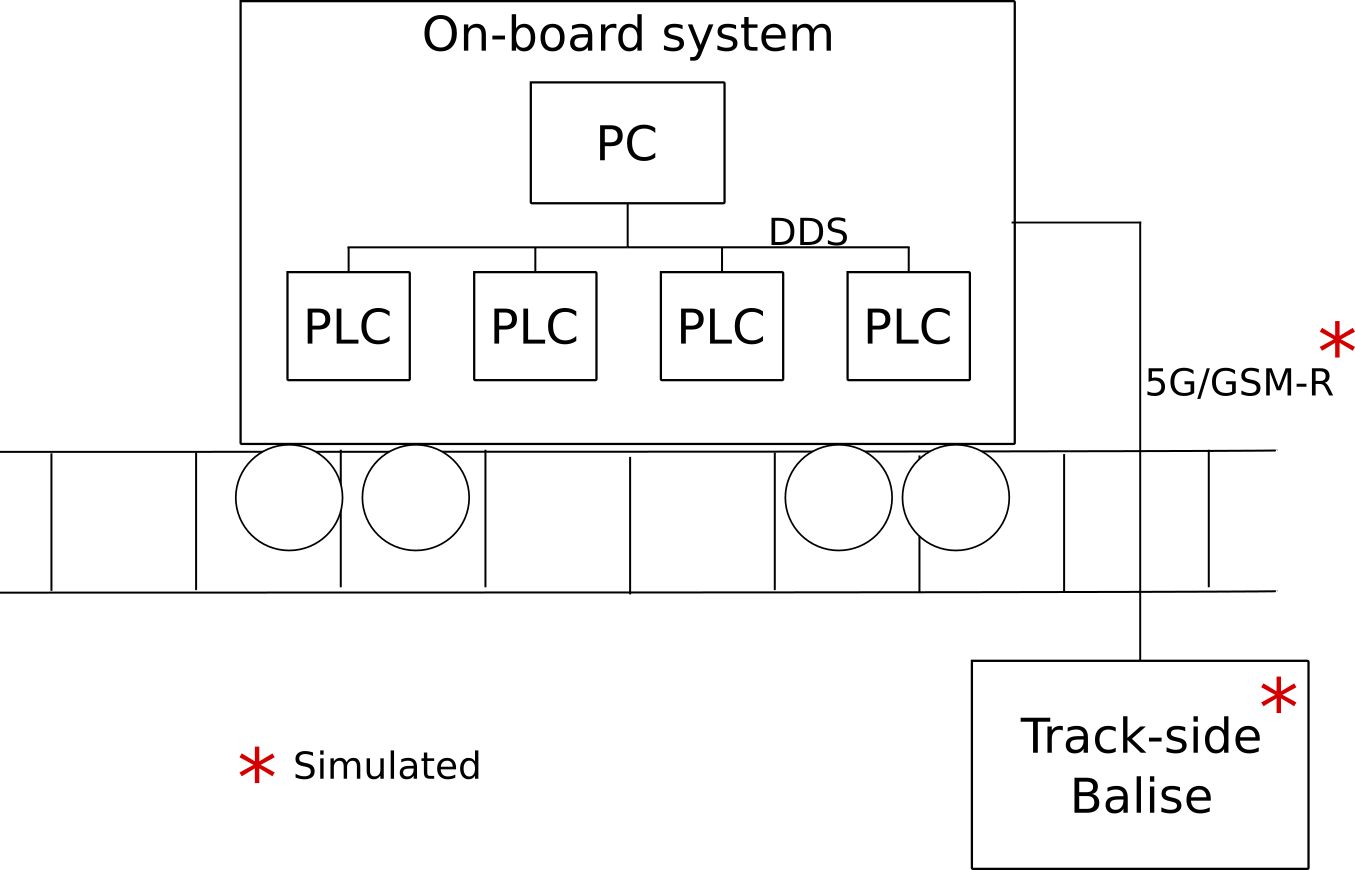
\includegraphics[width=\linewidth]{img/experimentalSetup.png}
  \caption{This work's experimental setup.}
  \label{fig:setup}
\end{figure}

The experimental setup is depicted in~\Autoref{fig:setup}.
It will comprise of a PC, a number of \glspl*{SPS}, an interconnect, a middleware layer running the \gls*{DDS} standard, and a simulation software.
The entire computation is done by the PC, which functions as the main computation unit but has no safety guarantees at all.
However, the \glspl*{SPS} feature a high-\gls*{SIL} \gls*{OS} and are used for redundancy computation by only reprocessing the workload's safety-critical parts.
Synchronizing the \gls*{SPS}'s results with the main PC supervises its work and wraps it into a safe envelope.
All \glspl*{SPS} are connected via an interconnect to the main PC.
By swapping out safety critical computations to the redundant working \glspl*{SPS} and sending data between individual components using the dependable real-time data exchange standard \gls*{DDS}, the entire system could be raised to a high \gls*{SIL}.

The simulation software imitates track-side balise as well as \gls*{RBC} components and their corresponding data telegrams and messages, which are received and evaluated by the PC and the four \glspl*{SPS}.
In order to facilitate a realistic test environment, the balise and \gls*{RBC} telegrams as well as the functional and operational principles are based on \gls*{ETCS} Subset-026.

The simulation software should also be deployable to a lab vehicle's on-board system.
In that case, it will use positioning information based on \gls*{GNSSINS} and odometry data of the lab vehicle in order to provide the system with virtual balise information.

% RELATED WORK
% -------------------------------------------------------------------------------------

\section*{Related Work}
Kugele et al. evaluate to what extend \gls*{DDS} is feasible for automotive software~\cite{KugeleDataCentricForAuto}.
For answering this question, they implement an automotive service-oriented architecture and perform benchmark experiments upon this architecture.
For evaluating \gls*{DDS}'s applicability in such a domain, Kugele et al. propose requirements and quality attributes for autonomous driving software.
The used list of requirements is composed by summarizing and adapting standards from the literature.
Their experiments are realized on a Ethernet topology with four Raspberry Pi 3 model B nodes and OpenDDS.
Results show that \gls*{DDS} provides decent yet expandable availability and safety characteristics.
However, they also state that \gls*{DDS} only covers automotive requirements when certain aspects, such as certification and security issues, are addressed.
Those aspects are not part of the \gls*{DDS} standard, though.
\\

Bijlsma et al. extend the state-of-the-art E-Gas layered monitoring concept to handle faults in a distributed and redundant system~\cite{DistributedSafety2020}.
Upon their middleware, \gls*{DDS} is applied to facilitate reliable communication among individual components with various \glspl*{ASIL}.
Besides functional data, diagnosis data is transmitted using \gls*{DDS} in order to detect faulty components.
\\

The applicability of the \gls*{DDS} standard and the OpenSplice DDS implementation for safety-critical railway systems is proven by Schmidt and van't Hag~\cite{SchmidtMissionCriticalChallenges}.
Findings show that OpenSplice DDS' \gls*{QOS} policies allow predictable time and locality characteristics for data distribution.
Further, this work provides and overview of \gls*{QOS} policies and OpenSplice DDS features to ensure reliability, availability, data-delivery, and resource usage.
Although Schmidt and van't Hag address OpenSplice DDS in their work, the results also apply to Cyclone DDS since it is designed as being a super-set of OpenSplice DDS.
\\

Jean-Louis Boulanger presents the 2011 version of the CENELEC 50128 standard and its implementations in his book~\cite{BoulangerStandards}.
CENELEC 50128 describes a software creation process for railway applications, as well as resources needed to achieve a set level of assurance.
Boulanger accentuates that the standard defines a context by which the safety of a software can be managed and thereby provides a guideline for safe software in the railway domain.


% WORK AND RISK ANALYSIS
% -------------------------------------------------------------------------------------

\section*{Work and Risk Analysis}
The project can be subdivided into four parts, namely the development of a train and track simulator, of a hardware setup, and of an on-board processing system, as well as a testing and evaluation phase.
This work's main part is the testing and evaluation phase, since this thesis' aim is to experimentally evaluate the system's functionality and reliability.
The on-board processing system, which is the foundation for the evaluation phase, comprises of data exchange with \gls*{DDS}, decision making, and redundant computation.
Designing, implementing, and evaluating the system's architecture and functional requirements is expected to take up the most time in this project.
Connecting the hardware is an essential part in this project but is unlikely to consume much time.
Simulating a train and track-side balises is chosen to be the show case of this work.
Because of \gls*{ETCS}'s complexity, building such a simulator from scratch is likely to take much resources.
It is preferred to either use existing simulators that provide the required packages or limit to basic and periodic messages at first and postpone the implementation of a train simulation to the end of this project.
For evaluating the system, it is not mandatory that the analyzed messages entirely conform to the \gls*{ETCS} specification, so that only a small part of \gls*{ETCS} will be covered by this project.

When possible, the final results should be tested on a lab vehicle.
This, however, depends on different external factors, such as time, admission, provision of the lab vehicle, and the vehicle's equipment.
If operating on a lab vehicle is not possible due to limitations in track-to-train communication, virtual balise telegrams could be used as an alternative.

\bibliographystyle{plain}
\bibliography{bibtex}

\printglossary
\end{document}
